% ============================================================================
% main.tex - HCMUT Graduation Thesis (English-Taught / High-Quality Program)
% Build order: pdflatex main -> bibtex main -> pdflatex main -> pdflatex main
% ============================================================================
\documentclass{hcmut-thesis}

% --- Thesis Cover & Sub-Cover Metadata ---
\upperuni{VIETNAM NATIONAL UNIVERSITY HO CHI MINH CITY}
\university{HO CHI MINH CITY UNIVERSITY OF TECHNOLOGY}
\faculty{FACULTY OF COMPUTER SCIENCE AND ENGINEERING}
\thesistype{GRADUATION THESIS}
\major{MAJOR: COMPUTER SCIENCE AND ENGINEERING}

\thesistitle{%
  DESIGN AND IMPLEMENTATION OF A FEDERATED LEARNING-BASED\\
  INTRUSION DETECTION AND PREVENTION SYSTEM\\
  WITH ZERO TRUST ARCHITECTURE AND SDN\\
  FOR HOSPITAL NETWORKS%
}

\advisor{Ph.D. Nguyễn Lê Duy Lai}

\students{%
  Nguyễn Đặng Minh Trường -- 2353262\\
  Lê Minh Hào -- 2310846\\
  Triệu Thuận Toàn -- 2353196%
}

\subcoverstudents{%
  Nguyễn Đặng Minh Trường -- 2353262\\
  Lê Minh Hào -- 2310846\\
  Triệu Thuận Toàn -- 2353196%
}

\place{HO CHI MINH CITY}
\dateyear{NOVEMBER 2026}

\begin{document}

% --- 1. Cover & Sub-Cover Pages ---
\hypersetup{pageanchor=false}
\makecoverpage
\makesubcoverpage
\hypersetup{pageanchor=true}

% --- 2. Front Matter (Roman Numerals) ---
\clearpage
\pagenumbering{roman}
\setcounter{page}{1}

\frontchapter{Graduation Thesis Task Assignment}

\noindent\textbf{VIETNAM NATIONAL UNIVERSITY HO CHI MINH CITY}\\
\textbf{HO CHI MINH CITY UNIVERSITY OF TECHNOLOGY}\\
\textbf{FACULTY OF COMPUTER SCIENCE AND ENGINEERING}

\vspace{0.5cm}
\begin{center}
  {\Large\bfseries GRADUATION THESIS TASK ASSIGNMENT}
\end{center}
\vspace{0.4cm}

\noindent\textbf{1. Students:}
\begin{itemize}[leftmargin=1.8em, nosep]
  \item Nguyễn Đặng Minh Trường -- Student ID: 2353262 -- Major: Computer Engineering (English-Taught Program)
  \item Lê Minh Hào -- Student ID: 2310846 -- Major: Computer Engineering (English-Taught Program)
  \item Triệu Thuận Toàn -- Student ID: 2353196 -- Major: Computer Engineering (English-Taught Program)
\end{itemize}

\vspace{0.3cm}
\noindent\textbf{2. Thesis Title:}\\
\textit{Design and Implementation of a Federated Learning-Based Intrusion Detection and Prevention System with Zero Trust Architecture and SDN for Hospital Networks.}

\vspace{0.3cm}
\noindent\textbf{3. Core Objectives and Scope:}
\begin{itemize}[leftmargin=1.8em, itemsep=4pt]
  \item \textbf{Core Hospital Network Infrastructure (Infrastructure as Code):} Design and deploy an enterprise three-tier Campus network topology (Core, Distribution, Access) using Cisco Catalyst/Nexus/ASA platforms, strict VLAN segmentation (Clinical zones, Paraclinical zones, Server Farm, DMZ, Out-of-Band Management, and SDN Control), VRF isolation, and automated deployment via Terraform/NetBox and Ansible.
  \item \textbf{Zero Trust Architecture \& SDN Enforcement (ZTA-SDN):} Enforce micro-segmentation across clinical, DMZ, and server zones; deploy Suricata IDS/IPS with SPAN traffic mirroring, OWASP ModSecurity CRS WAF, Policy Enforcement Points (PEPs), and an SDN Controller (Ryu/Faucet/OpenFlow) acting as the Policy Decision Point (PDP) for dynamic quarantining and flow-rule enforcement.
  \item \textbf{Federated Learning Intrusion Detection (FL-IDS):} Design and train lightweight deep learning models (such as 1D-CNN, MLP, or CNN-BiLSTM) under Federated Learning (Flower/FedAvg) across distributed hospital edge nodes (DMZ, Clinical, Paraclinical) without centralizing raw patient-adjacent network traffic.
  \item \textbf{Closed-Loop Integration \& Evaluation:} Couple the FL-IDS detection engine with the SDN Policy Engine and verify end-to-end attack mitigation latency, classification accuracy, and false-positive behavior under realistic hospital workloads.
\end{itemize}

\vspace{0.3cm}
\noindent\textbf{4. Deliverables and Schedule:}
\begin{itemize}[leftmargin=1.8em, nosep]
  \item Hardcopy and softcopy of the Graduation Thesis report in English according to HCMUT Faculty of Computer Science and Engineering regulations.
  \item Reproducible Infrastructure-as-Code repository, FL-IDS training/inference pipeline, ZTA-SDN policy engine, and benchmark testbed artifacts.
  \item Assignment Issue Date: \texttt{[DD/MM/2026]} \hfill Submission Date: \texttt{[DD/MM/2026]}
\end{itemize}

\vspace{1.2cm}
\noindent
\begin{minipage}[t]{0.48\textwidth}
  \centering
  \textbf{FACULTY DEAN / DEPARTMENT CHAIR}\\[2.2cm]
  \textit{(Signature and full name)}
\end{minipage}
\hfill
\begin{minipage}[t]{0.48\textwidth}
  \centering
  Ho Chi Minh City, \texttt{[DD/MM/2026]}\\
  \textbf{THESIS ADVISOR}\\[2.2cm]
  \textbf{Ph.D. Nguyễn Lê Duy Lai}
\end{minipage}

\frontchapter{Declaration of Authorship}

We hereby declare that this graduation thesis, entitled \textit{``Design and Implementation of a Federated Learning-Based Intrusion Detection and Prevention System with Zero Trust Architecture and SDN for Hospital Networks''}, is our own original work conducted under the supervision of \textbf{Ph.D. Nguyễn Lê Duy Lai} at the Faculty of Computer Science and Engineering, Ho Chi Minh City University of Technology -- Vietnam National University Ho Chi Minh City.

All network designs, automation playbooks, Software-Defined Networking (SDN) policies, Federated Learning scripts, and experimental results presented in this thesis are honestly developed, deployed, and measured by our team on our research testbed. All prior studies, open-source software, reference architectures, datasets, and technical documents used in this work are properly cited and listed in the References section. We take full responsibility before the University and the Defense Committee for the accuracy and integrity of this work.

\vspace{1.5cm}
\noindent\hfill
\begin{minipage}{0.55\textwidth}
  \centering
  Ho Chi Minh City, November 2026\\[0.2cm]
  \textbf{Authors}\\[0.6cm]
  \begin{tabular}{@{}l@{\hspace{1.2cm}}c@{}}
    Nguyễn Đặng Minh Trường & \textit{(Signature)} \\[0.6cm]
    Lê Minh Hào & \textit{(Signature)} \\[0.6cm]
    Triệu Thuận Toàn & \textit{(Signature)}
  \end{tabular}
\end{minipage}

\frontchapter{Acknowledgments}

First and foremost, we would like to express our deepest gratitude to \textbf{Ph.D. Nguyễn Lê Duy Lai}, our thesis advisor at the Faculty of Computer Science and Engineering, Ho Chi Minh City University of Technology -- VNU-HCM. Throughout our graduation research, he has provided invaluable academic guidance, insightful feedback on security architecture and Federated Learning methodology, and continuous encouragement that helped us overcome complex engineering challenges.

We sincerely thank all lecturers and staff of the Faculty of Computer Science and Engineering and the Office for International Study Programs (OISP) for equipping us with a rigorous foundation in computer engineering, networking, and systems security during our undergraduate studies.

We are also grateful to our families and friends for their unwavering support, patience, and motivation throughout the completion of this thesis. Finally, we appreciate the mutual collaboration within our research group, whose collective dedication made the design, automation, and experimental evaluation of this hospital network security platform possible.

\frontchapter{Abstract}

Modern hospital networks interconnect heterogeneous endpoints across clinical departments, diagnostic imaging equipment, Internet of Medical Things (IoMT) sensors, enterprise servers, and public-facing patient portals. Traditional perimeter-based security architectures rely on static firewall rules and implicit internal trust, leaving healthcare infrastructures vulnerable to lateral movement once a single endpoint or medical device is compromised. Furthermore, centralizing raw clinical network traffic for Artificial Intelligence (AI)-driven intrusion detection raises significant privacy and regulatory compliance risks while introducing bandwidth bottlenecks.

To address these challenges, this graduation thesis presents the design and implementation of a \textbf{Federated Learning-based Intrusion Detection and Prevention System integrated with Zero Trust Architecture and Software-Defined Networking (FL-IDS + ZTA-SDN)} for hospital networks. The proposed architecture comprises three tightly coupled layers:
\begin{enumerate}[leftmargin=1.8em, itemsep=4pt]
  \item \textbf{Segmented Hospital Infrastructure via Infrastructure as Code (IaC):} A three-tier Campus network topology (Core, Distribution, Access) managed with Cisco Catalyst, Nexus, and ASA platforms, featuring strict VLAN micro-segmentation across clinical, paraclinical, server farm, DMZ, and Out-of-Band (OOB) management zones, VRF isolation, and automated provisioning through NetBox, Terraform, and Ansible.
  \item \textbf{Zero Trust Policy Enforcement and SDN Control:} Continuous verification governed by a centralized Policy Decision Point (PDP) and SDN Controller that dynamically adjusts OpenFlow rules on Policy Enforcement Points (PEPs), complemented by OWASP ModSecurity CRS at the DMZ Web Application Firewall and Suricata IDS/IPS inspecting mirrored SPAN traffic.
  \item \textbf{Privacy-Preserving Federated Learning IDS:} Distributed local intrusion detection models trained at hospital edge zones using the FedAvg aggregation protocol, enabling collaborative multi-department threat intelligence without exposing raw sensitive traffic outside local boundaries.
\end{enumerate}

The integrated system forms a closed-loop security pipeline---from edge packet inspection and federated classification to automated SDN quarantine and micro-segmentation enforcement---aiming to achieve high detection accuracy ($>95\%$ target benchmark in Chapter~5 evaluation), low false-positive rates, and rapid automated containment while preserving patient data privacy.

\vspace{0.5cm}
\noindent\textbf{Keywords:} Hospital Network Security, Zero Trust Architecture (ZTA), Software-Defined Networking (SDN), Federated Learning (FL), Intrusion Detection and Prevention System (IDS/IPS), Infrastructure as Code (IaC).

\frontchapter{Tóm tắt}

Mạng bệnh viện hiện đại kết nối nhiều loại thiết bị đa dạng giữa các khoa lâm sàng, hệ thống chẩn đoán hình ảnh, thiết bị Y tế Kết nối (IoMT), cụm máy chủ nội bộ (HIS, PACS, LIS) và cổng thông tin bệnh nhân tại vùng DMZ. Các mô hình bảo mật truyền thống dựa trên vành đai tường lửa tĩnh và sự tin cậy mặc định bên trong mạng nội bộ không còn đủ khả năng ngăn chặn sự lây lan ngang (lateral movement) khi một thiết bị đầu cuối bị xâm nhập. Bên cạnh đó, việc thu thập tập trung dữ liệu lưu lượng mạng để huấn luyện các mô hình Học sâu phát hiện xâm nhập đặt ra rủi ro lớn về quyền riêng tư dữ liệu bệnh nhân và gây quá tải băng thông đường truyền.

Để giải quyết bài toán trên, luận văn này đề xuất thiết kế và hiện thực một \textbf{Hệ thống Phát hiện và Ngăn chặn Xâm nhập dựa trên Học liên kết (Federated Learning), kết hợp Kiến trúc Không tin cậy (Zero Trust Architecture) và Mạng Điều khiển bằng Phần mềm (SDN)} cho hạ tầng mạng bệnh viện. Hệ thống được tổ chức theo ba lớp gắn kết chặt chẽ:
\begin{enumerate}[leftmargin=1.8em, itemsep=4pt]
  \item \textbf{Hạ tầng mạng bệnh viện phân mảnh theo hướng Infrastructure as Code (IaC):} Xây dựng kiến trúc mạng Campus ba tầng (Core, Distribution, Access) với phân chia VLAN chặt chẽ theo từng phân khu (Lâm sàng, Cận lâm sàng, Máy chủ, DMZ, Quản trị Out-of-Band), cô lập VRF và tự động hóa triển khai qua NetBox, Terraform và Ansible.
  \item \textbf{Thực thi Zero Trust và điều khiển SDN:} Tích hợp tường lửa ứng dụng Web OWASP CRS tại DMZ, hệ thống phát hiện xâm nhập Suricata thông qua cơ chế nhân bản lưu lượng SPAN, kết hợp với bộ điều khiển SDN đóng vai trò điểm quyết định chính sách (PDP) để tự động cô lập thiết bị bất thường theo thời gian thực.
  \item \textbf{Phát hiện xâm nhập bảo toàn riêng tư bằng Học liên kết (FL-IDS):} Huấn luyện mô hình học sâu cục bộ tại các nút biên (DMZ, Lâm sàng, Cận lâm sàng) và chỉ chia sẻ tham số trọng số về máy chủ tổng hợp thông qua giao thức FedAvg, đảm bảo dữ liệu thô không rời khỏi phân vùng cục bộ.
\end{enumerate}

Hệ thống hướng đến một vòng lặp bảo mật khép kín từ giám sát lưu lượng, phát hiện bất thường đến tự động cách ly luồng độc hại, đạt mục tiêu độ chính xác phát hiện cao ($>95\%$ trong kịch bản đánh giá ở Chương~5), tỷ lệ cảnh báo giả thấp và thời gian phản ứng nhanh trong khi vẫn đảm bảo an toàn thông tin y tế.

\vspace{0.5cm}
\noindent\textbf{Từ khóa:} Bảo mật mạng bệnh viện, Kiến trúc Không tin cậy (ZTA), Mạng Điều khiển bằng Phần mềm (SDN), Học liên kết (FL), Hệ thống Phát hiện và Ngăn chặn Xâm nhập (IDS/IPS), Infrastructure as Code (IaC).


\clearpage
\tableofcontents
\addcontentsline{toc}{chapter}{Table of Contents}

\clearpage
\listoffigures
\addcontentsline{toc}{chapter}{List of Figures}

\clearpage
\listoftables
\addcontentsline{toc}{chapter}{List of Tables}

\frontchapter{List of Abbreviations and Acronyms}

\noindent
\begin{longtable}{@{}p{3.4cm}p{10.8cm}@{}}
\toprule
\textbf{Acronym / Term} & \textbf{Full Form / Definition} \\
\midrule
\endfirsthead
\toprule
\textbf{Acronym / Term} & \textbf{Full Form / Definition} \\
\midrule
\endhead
\bottomrule
\endfoot
ACL & Access Control List \\
AD / LDAP & Active Directory / Lightweight Directory Access Protocol \\
AI & Artificial Intelligence \\
ASA & Cisco Adaptive Security Appliance \\
BGP & Border Gateway Protocol \\
BiLSTM & Bidirectional Long Short-Term Memory \\
CRS & OWASP Core Rule Set \\
DHCP & Dynamic Host Configuration Protocol \\
DICOM & Digital Imaging and Communications in Medicine \\
DMZ & Demilitarized Zone \\
DNS & Domain Name System \\
DL & Deep Learning \\
EMR / EHR & Electronic Medical Record / Electronic Health Record \\
FedAvg & Federated Averaging \\
FL & Federated Learning \\
FL-IDS & Federated Learning-based Intrusion Detection System \\
GLBP & Gateway Load Balancing Protocol \\
HIS & Hospital Information System \\
HL7 / FHIR & Health Level Seven / Fast Healthcare Interoperability Resources \\
HSRP & Hot Standby Router Protocol \\
IaC & Infrastructure as Code \\
ICMP & Internet Control Message Protocol \\
ICU & Intensive Care Unit \\
IDS / IPS & Intrusion Detection System / Intrusion Prevention System \\
IoMT & Internet of Medical Things \\
LIS & Laboratory Information System \\
ML & Machine Learning \\
MQTT & Message Queuing Telemetry Transport \\
NAT & Network Address Translation \\
NetBox & Open-source IPAM and Data Center Infrastructure Management (DCIM) Source of Truth \\
OOB & Out-of-Band (Management Network -- VLAN 999) \\
OSPF & Open Shortest Path First \\
OVS & Open vSwitch \\
PACS & Picture Archiving and Communication System \\
PAT & Port Address Translation \\
PDP & Policy Decision Point \\
PEP & Policy Enforcement Point \\
RBAC & Role-Based Access Control \\
REST API & Representational State Transfer Application Programming Interface \\
RSPAN / SPAN & Remote Switch Port Analyzer / Switch Port Analyzer \\
SDN & Software-Defined Networking \\
SIEM & Security Information and Event Management \\
SSH & Secure Shell \\
SVI & Switched Virtual Interface \\
VLAN & Virtual Local Area Network \\
VRF & Virtual Routing and Forwarding \\
WAF & Web Application Firewall \\
ZTA & Zero Trust Architecture \\
\end{longtable}


% --- 3. Main Body (Arabic Numerals) ---
\clearpage
\pagenumbering{arabic}
\setcounter{page}{1}

\chapter{Introduction}
\label{ch:introduction}

\section{Background and Motivation}
\label{sec:background}

Modern healthcare delivery depends heavily on interconnected digital infrastructure. Hospitals routinely operate heterogeneous environments linking Hospital Information Systems (HIS), Electronic Medical Records (EMR), Picture Archiving and Communication Systems (PACS), Laboratory Information Systems (LIS), clinical workstations, web-based patient portals, and constrained Internet of Medical Things (IoMT) devices such as infusion pumps, patient monitors, and diagnostic scanners. While digital connectivity improves clinical workflows and diagnostic turnaround, it also exposes life-critical infrastructure to severe cyber threats, including ransomware, credential harvesting, medical device exploitation, and unauthorized exfiltration of protected health information.

Historically, enterprise and campus hospital networks relied on perimeter-based security models centered on hierarchical switching, static Access Control Lists (ACLs), and border firewalls~\cite{ciscoCampusArchitecture,ciscoHealthcareProfile}. In such perimeter-centric designs, devices inside the trusted internal boundary are often granted implicit trust, allowing an attacker who compromises a single clinical workstation or public-facing service to perform reconnaissance and lateral movement toward high-value assets such as PACS archives or HIS databases. Furthermore, legacy manual network provisioning across multi-tier switches introduces configuration drift, inconsistent VLAN segmentation, and slow incident containment.

To resolve these structural weaknesses, Zero Trust Architecture (ZTA), as formalized in NIST SP 800-207~\cite{rose2020zerotrust}, eliminates implicit trust based on network location. ZTA requires continuous verification, least-privilege access, and granular micro-segmentation enforced dynamically at Policy Enforcement Points (PEPs) under the direction of a Policy Decision Point (PDP). When paired with Software-Defined Networking (SDN)~\cite{onfSdnDefinition}, the decoupled control plane can inspect telemetry, evaluate risk context, and programmatically install or revoke flow rules across switches to quarantine compromised endpoints in real time~\cite{xu2025zero}.

At the same time, static signature-based intrusion detection struggles against zero-day exploits and evolving attack vectors. Deep Learning-based Intrusion Detection Systems (DL-IDS) improve anomaly recognition, yet training centralized models requires aggregating raw traffic logs across hospital departments. In healthcare, raw packet captures and flow records may carry sensitive clinical metadata and strain inter-departmental links. Federated Learning (FL), introduced via the FedAvg algorithm~\cite{mcmahan2017communication}, offers a privacy-preserving alternative: distributed hospital edge nodes train intrusion detection models locally and exchange only model weight updates with a central aggregation server~\cite{javeed2024federated,amiri2023sids}. Combining FL-IDS with ZTA-SDN therefore establishes a unified, privacy-preserving, and self-defending hospital network architecture~\cite{alanazi2026edgeguard,khan2025integrating}.

\section{Problem Statement}
\label{sec:problem_statement}

Despite recent advances in SDN security and Federated Learning, deploying a practical intrusion detection and prevention architecture in realistic hospital networks presents four key challenges:

\begin{enumerate}[leftmargin=1.8em, itemsep=6pt]
  \item \textbf{Lack of Deterministic Segmentation and Reproducible Provisioning:} Hospital campuses combine high-risk public zones (DMZ), sensitive clinical departments, legacy IoMT endpoints, and core server farms. Manual CLI configuration of VLANs, VRFs, routing protocols, and Out-of-Band (OOB) management protection is error-prone and difficult to audit under Zero Trust principles~\cite{ciscoHealthcareProfile}.
  \item \textbf{Insufficient East-West Visibility and Static Perimeter Defense:} Perimeter firewalls alone cannot inspect or contain malicious lateral traffic once an internal clinical workstation or DMZ application server is breached~\cite{rose2020zerotrust}. Effective enforcement requires out-of-band SPAN traffic mirroring~\cite{ciscoSpan} paired with inline/passive inspection~\cite{suricataIpsConcept,owasp2026crs} and dynamic SDN flow revocation.
  \item \textbf{Privacy and Bandwidth Constraints in Multi-Department AI Training:} Centralizing raw traffic datasets from multiple hospital wards or partner clinics violates data-minimization principles and creates heavy ingestion overhead~\cite{javeed2024federated,amiri2023sids}. An IDS must learn across heterogeneous traffic profiles (e.g., HTTP/HTTPS in the DMZ versus DICOM/HL7 in clinical wards) without centralizing raw packets.
  \item \textbf{Disconnection Between Detection and Automated Enforcement:} Many FL-IDS proposals evaluate offline classification accuracy without closing the control loop back to programmable network Policy Enforcement Points~\cite{xu2025zero,alanazi2026edgeguard}. Without low-latency PDP/PEP integration, alerts require manual operator intervention while threats continue to propagate.
\end{enumerate}

\section{Research Objectives}
\label{sec:objectives}

To address the challenges above, this thesis designs, implements, and evaluates a cohesive three-layer hospital network security platform with the following concrete objectives:

\begin{itemize}[leftmargin=1.8em, itemsep=6pt]
  \item \textbf{Objective 1 -- Automated Segmented Campus Infrastructure (IaC):} Build an automated three-tier hospital network topology (Core, Distribution, Access) with isolated VRFs, granular clinical/server/DMZ/OOB VLANs, redundant first-hop gateways (HSRP/GLBP), and reproducible deployment via NetBox, Terraform, and Ansible.
  \item \textbf{Objective 2 -- Zero Trust Micro-Segmentation and SDN Policy Engine:} Implement strict east-west ACLs, OOB management plane hardening, OWASP ModSecurity CRS protection on DMZ web portals~\cite{owasp2026crs}, Suricata IDS/IPS inspection over SPAN sessions~\cite{ciscoSpan,suricataIpsConcept}, and a PDP/SDN controller capable of dynamically enforcing quarantine policies on PEPs.
  \item \textbf{Objective 3 -- Privacy-Preserving Federated Learning IDS:} Develop and train lightweight deep neural intrusion detection models across distributed hospital edge nodes (DMZ, Clinical, and Paraclinical sensors) using Federated Averaging (FedAvg)~\cite{mcmahan2017communication} without transferring raw traffic logs outside local zones.
  \item \textbf{Objective 4 -- Closed-Loop Evaluation and Performance Benchmarking:} Integrate the FL-IDS inference stream with the ZTA-SDN control plane and benchmark detection performance (targeting $>95\%$ classification accuracy in Chapter~5 evaluation), false-positive rate, communication overhead, and end-to-end mitigation latency against simulated cyberattack scenarios.
\end{itemize}

\section{System Architecture and Implementation Scope}
\label{sec:scope}

Figure~\ref{fig:system_architecture} illustrates the end-to-end architecture constructed in this thesis, spanning the Hospital Campus data plane, the ZTA-SDN enforcement and inspection plane, and the Federated Learning plane.

\begin{figure}[htbp]
  \centering
  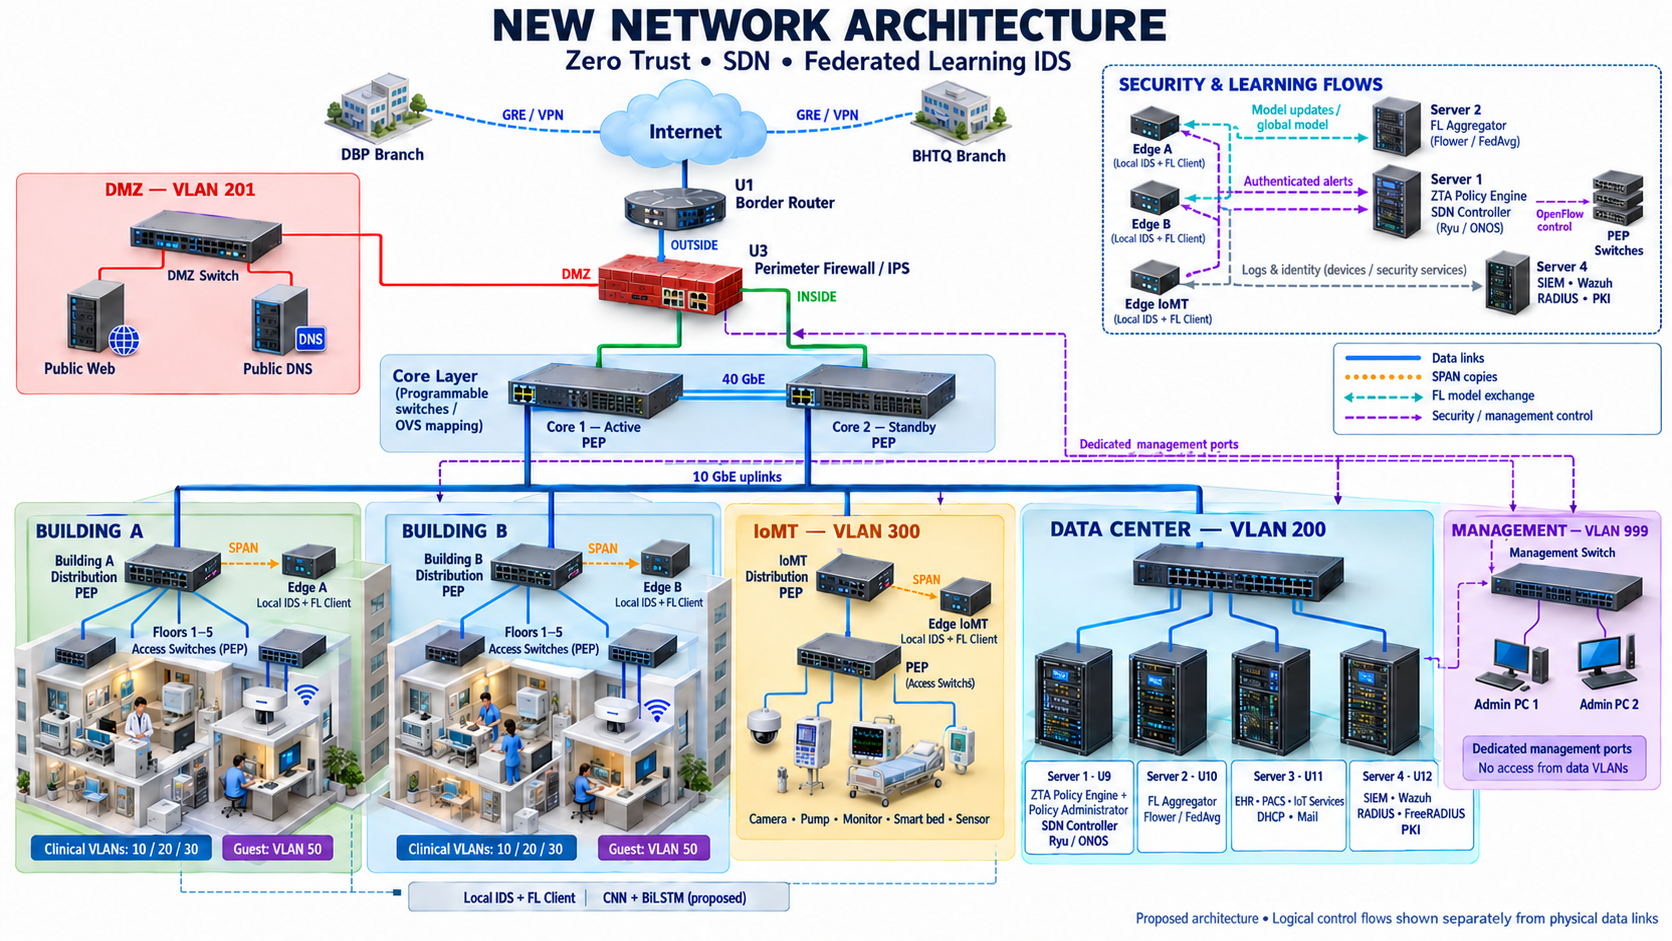
\includegraphics[width=0.96\textwidth]{graphics/architecture-overview.png}
  \caption{Overall FL-IDS + ZTA-SDN architecture for the segmented hospital network.}
  \label{fig:system_architecture}
\end{figure}

Within this graduation thesis, the system scope is structured into clear hardware/virtualization boundaries and departmental security zones, summarized in Table~\ref{tab:vlan_zones}.

\begin{table}[htbp]
  \centering
  \caption{Logical hospital network segmentation across zones and VRFs.}
  \label{tab:vlan_zones}
  \begin{tabular}{@{}l l l p{5.8cm}@{}}
    \toprule
    \textbf{Zone / VRF} & \textbf{VLAN IDs} & \textbf{Subnet Range} & \textbf{Primary Role and Security Policy} \\
    \midrule
    Clinical Zone & 10, 20, 30, 50, 60, 80 & \texttt{10.10.x.0/24} & Reception, Doctors, ICU, Wards, Pediatrics, Outpatient EMR clients; OOB access blocked via ingress ACLs. \\
    Paraclinical Zone & 110, 120, 130 & \texttt{10.20.x.0/24} & Laboratory, Diagnostic Imaging (PACS/DICOM), Pharmacy terminals; restricted server-only flows. \\
    Server Farm & 210, 220, 230, 240 & \texttt{10.30.x.0/24} & HIS/EMR app servers, PACS/LIS storage, Identity (AD/LDAP), SIEM/Monitoring. \\
    DMZ & 310, 320 & \texttt{172.16.x.0/24} & Patient Web Portal, OWASP CRS WAF, Reverse Proxy, DMZ IDS/FL edge sensor. \\
    SDN Control & 400 & \texttt{10.40.0.0/24} & OpenFlow control plane, PDP policy engine, FL aggregation server. \\
    OOB Management & 999 & \texttt{10.99.99.0/24} & Isolated device SSH management, NetBox/Ansible automation node, Tailscale bastion. \\
    \bottomrule
  \end{tabular}
\end{table}

\textbf{Scope Boundaries:}
\begin{itemize}[leftmargin=1.8em, itemsep=4pt]
  \item \textbf{Testbed Emulation:} The network core, distribution, access switches, edge firewall, and Linux service servers are emulated in GNS3 and VMware virtualized hosts using enterprise-representative images (Cisco IOSv/IOSvL2, ASAv, and Ubuntu Linux) with Infrastructure-as-Code pipelines stored in the project repository (\texttt{hospital-zta-sdn-fl}).
  \item \textbf{Detection and Mitigation Focus:} The FL-IDS evaluates both standard benchmark intrusion datasets and synthetic hospital-like attack traffic (e.g., port scanning, brute-force SSH, web exploitation, DICOM/clinical lateral movement). Compliance auditing is scoped to technical network/system controls rather than legal hospital accreditation.
\end{itemize}

\section{Contributions of the Thesis}
\label{sec:contributions}

The principal engineering and research contributions of this thesis are summarized as follows:

\begin{enumerate}[leftmargin=1.8em, itemsep=6pt]
  \item \textbf{Reproducible Zero-Touch Hospital Campus Infrastructure:} Designing a complete three-tier segmented hospital network backed by a single Source of Truth (NetBox), Terraform orchestration, and idempotent Ansible roles covering multi-VRF routing, two-layer OOB management protection, DNS/DHCP/Identity services, and OWASP CRS WAF deployment.
  \item \textbf{Integrated ZTA-SDN Enforcement and Out-of-Band Visibility:} Bridging enterprise Cisco SPAN traffic mirroring~\cite{ciscoSpan} and Suricata IDS/IPS~\cite{suricataIpsConcept} with an SDN Policy Decision Point that dynamically enforces quarantine and least-privilege rules at Policy Enforcement Points in alignment with NIST SP 800-207~\cite{rose2020zerotrust}.
  \item \textbf{Privacy-Preserving Multi-Zone FL-IDS Pipeline:} Implementing a federated intrusion detection workflow across logically isolated hospital domains (DMZ, Clinical, Paraclinical) using FedAvg~\cite{mcmahan2017communication} so collaborative detection improves without centralizing raw clinical network traffic~\cite{javeed2024federated,amiri2023sids}.
  \item \textbf{End-to-End Closed-Loop Validation Framework:} Delivering an automated, reproducible experimental testbed capable of quantifying classification accuracy, non-IID federated convergence, and real-time SDN quarantine latency under realistic attack scenarios.
\end{enumerate}

\section{Thesis Organization}
\label{sec:organization}

The remainder of this thesis is organized into five chapters:

\begin{itemize}[leftmargin=1.8em, itemsep=5pt]
  \item \textbf{Chapter~2 -- Theoretical Background and Infrastructure Design:} Reviews Zero Trust Architecture (NIST SP 800-207), SDN architecture, enterprise three-tier Campus design, IDS/IPS and WAF principles, Federated Learning foundations, and details our IaC-driven hospital network implementation.
  \item \textbf{Chapter~3 -- Federated Learning-Based Intrusion Detection System (FL-IDS):} Presents the deep learning model architecture, feature engineering over hospital and benchmark flow data, distributed FedAvg training pipeline, and edge inference design.
  \item \textbf{Chapter~4 -- Zero Trust Architecture and SDN Integration:} Details the coupling of Suricata/SPAN telemetry and FL-IDS alerts with the SDN PDP/PEP control loop, dynamic quarantine workflows, and policy enforcement rules.
  \item \textbf{Chapter~5 -- Experiments and Evaluation:} Describes the integrated testbed setup, attack simulation scenarios, FL-IDS classification benchmarks, SDN enforcement latency measurements, and comparative analysis.
  \item \textbf{Chapter~6 -- Conclusion and Future Work:} Summarizes key findings, discusses system limitations, and outlines future extensions for production healthcare deployments.
\end{itemize}

\chapter{Theoretical Background and Hospital Infrastructure Design}
\label{ch:theoretical_background}

% [TODO - Chapter Owner: Member 1 & Lead]
% Write full prose expanding each subsection below based on verified repository artifacts
% (ansible/, terraform/, netbox/, topology) and references.bib citations.

\section{Hospital Network Characteristics and Security Challenges}
\label{sec:hospital_challenges}
% Cover HIS, EMR, PACS, LIS, IoMT endpoints, HIPAA/data-privacy requirements, and
% risks of lateral movement under flat or perimeter-only network topologies.

\section{Zero Trust Architecture (NIST SP 800-207)}
\label{sec:zta_theory}
% Cover ZTA core tenets, Policy Engine / Policy Administrator (PDP), Policy Enforcement
% Point (PEP), trust algorithms, and micro-segmentation principles (\cite{rose2020zerotrust}).

\section{Software-Defined Networking (SDN)}
\label{sec:sdn_theory}
% Cover decoupling of control and data planes, OpenFlow southbound protocol, Open vSwitch
% (OVS), SDN controller (Ryu/Faucet), and programmable flow rules (\cite{onfSdnDefinition,xu2025zero}).

\section{Intrusion Detection, Prevention, and Web Application Firewalls}
\label{sec:ids_waf_theory}
% Cover signature vs. anomaly-based IDS/IPS, Suricata inspection over SPAN/RSPAN mirroring
% (\cite{ciscoSpan,suricataIpsConcept}), and OWASP ModSecurity CRS (\cite{owasp2026crs}).

\section{Federated Learning Foundations}
\label{sec:fl_theory}
% Cover FedAvg (\cite{mcmahan2017communication}), client-server aggregation rounds, non-IID
% departmental data distributions, and privacy advantages in FL-IDS (\cite{javeed2024federated,amiri2023sids}).

\section{Hospital Campus Network Architecture and IaC Implementation}
\label{sec:campus_iac_design}
% Detail our implemented 3-tier Campus topology (Core, Distribution, Access, Cisco ASAv),
% VRF isolation, Clinical/Paraclinical/Server/DMZ/SDN/OOB VLANs, two-layer OOB protection
% (CLINICAL_PROTECT_OOB & OOB_VTY_ONLY), and NetBox/Terraform/Ansible automation pipelines
% (\cite{ciscoCampusArchitecture,ciscoHealthcareProfile}).

\chapter{Federated Learning-Based Intrusion Detection System}
\label{ch:fl_ids}

% [TODO - Chapter Owner: AI / FL Team Member]
% Implement and document Phase 3 FL-IDS design, datasets, preprocessing, neural models,
% FedAvg aggregation pipeline, and alert output schema.

\section{FL-IDS Architecture in the Hospital Topology}
\label{sec:fl_architecture}
% Explain placement of FL clients at edge sensors (DMZ, Clinical, Paraclinical) and the
% FL aggregation server inside VLAN 400 / Server management segment.

\section{Datasets and Feature Engineering}
\label{sec:fl_datasets}
% Document benchmark datasets (e.g., CIC-IDS2017 / NSL-KDD / BoT-IoT / synthetic hospital
% flows), feature selection, normalization, class-imbalance handling, and non-IID partitioning.

\section{Deep Learning Detection Model Design}
\label{sec:fl_model}
% Present model architecture (e.g., 1D-CNN, MLP, or CNN-BiLSTM following \cite{javeed2024federated}),
% hyperparameters, loss function, and lightweight inference considerations for edge sensors.

\section{Federated Training and Aggregation Protocol}
\label{sec:fl_training}
% Detail Flower / PyTorch FedAvg workflow, communication rounds, local epochs, weight
% serialization, and convergence behavior without raw packet sharing (\cite{mcmahan2017communication}).

\section{Alert Generation and Interface to the Policy Engine}
\label{sec:fl_alert_interface}
% Define JSON/syslog alert schema (source IP, target VLAN, attack class, confidence score)
% pushed to the ZTA-SDN Policy Decision Point (PDP).

\chapter{Zero Trust Architecture and SDN Integration}
\label{ch:zta_sdn_integration}

% [TODO - Chapter Owner: Network / SDN Team Member]
% Document Phase 2 ZTA-SDN enforcement plane: SPAN mirroring, Suricata/WAF telemetry,
% Trust Engine / PDP logic, SDN Controller flow installation, and automated containment.

\section{Control and Data Plane Integration Topology}
\label{sec:zta_sdn_topology}
% Show how Cisco distribution/access SPAN traffic feeds Suricata and FL sensors, and how
% OpenFlow PEPs (OVS bridges / SDN switches) enforce traffic policies in VLAN 400.

\section{Policy Decision Point (PDP) and Trust Scoring Engine}
\label{sec:pdp_trust_engine}
% Formulate trust score evaluation combining device identity (AD/LDAP/NetBox), zone
% context, OWASP CRS alerts, Suricata signatures, and FL-IDS anomaly confidence (\cite{xu2025zero}).

\section{Policy Enforcement Points (PEPs) and Dynamic Flow Control}
\label{sec:pep_flow_control}
% Describe OpenFlow rules installed by the SDN Controller: allow, rate-limit, redirect to
% honeypot/inspection, and dynamic host quarantine.

\section{Closed-Loop Automated Incident Response Workflow}
\label{sec:closed_loop_workflow}
% Trace the end-to-end closed loop from packet capture -> inference -> trust degradation ->
% SDN flow drop/quarantine -> SIEM logging (\cite{alanazi2026edgeguard,khan2025integrating}).

\chapter{Experiments and Evaluation}
\label{ch:experiments_evaluation}

% [TODO - Chapter Owner: Full Team]
% Populate all experimental setup tables, confusion matrices, ROC/accuracy curves, latency
% measurements, and ablation comparisons once Phase 2 & Phase 3 testbed runs are complete.

\section{Experimental Testbed and Attack Scenarios}
\label{sec:testbed_scenarios}
% Document hardware/VM specs (VMware, GNS3, OVS, Ubuntu servers), traffic generators, and
% test scenarios (port scan, SSH brute-force, SQLi/XSS against Patient Portal, lateral pivot).

\section{FL-IDS Classification Performance}
\label{sec:eval_fl_metrics}
% [TODO] Report Accuracy (target benchmark >95%), Precision, Recall, F1-Score, FPR, and
% per-class confusion matrices comparing Centralized vs. Local-Only vs. FedAvg training.

\section{Federated Convergence and Resource Overhead}
\label{sec:eval_convergence}
% [TODO] Measure global loss/accuracy across FedAvg rounds under IID and non-IID zone splits,
% CPU/RAM footprint on edge VMs, and model weight transmission overhead.

\section{ZTA-SDN Enforcement Latency and Mitigation Effectiveness}
\label{sec:eval_sdn_latency}
% [TODO] Measure detection-to-quarantine latency (t_detect -> t_pdp -> t_openflow),
% throughput impact on benign HIS/PACS flows, and verification of OOB/VRF isolation.

\section{Comparison with Existing Approaches}
\label{sec:eval_comparison}
% [TODO] Benchmark qualitatively and quantitatively against related works
% (\cite{javeed2024federated,xu2025zero,alanazi2026edgeguard,amiri2023sids}).

\chapter{Conclusion and Future Work}
\label{ch:conclusion}

% [TODO - Chapter Owner: Lead & Full Team]
% Finalize after Chapter 5 results are collected.

\section{Summary of Achievements}
\label{sec:summary_achievements}
% Summarize completed deliverables across Step 1 (IaC hospital network), Step 2 (ZTA-SDN),
% and Step 3 (FL-IDS), referencing verified measurements from Chapter 5.

\section{Limitations}
\label{sec:limitations}
% Discuss virtualized testbed constraints vs. physical medical IoMT hardware, encrypted TLS
% payload visibility boundaries, and federated poisoning resilience gaps.

\section{Future Directions}
\label{sec:future_work}
% Outline differential privacy / secure aggregation for FL updates, Byzantine-robust
% aggregation, encrypted traffic behavioral fingerprinting, and hardware P4/SDN offload.


% --- 4. References ---
\clearpage
\addcontentsline{toc}{chapter}{References}
\bibliographystyle{IEEEtran}
\bibliography{references}

\end{document}
